
\section{Состояние атмосферы}
\begin{frame}{\insertsectionhead}
    \footnotesize
    По информации из ежемесячных отчётов по качеству
    атмосферного воздуха\cite{goveco}, с февраля 2017 года
    по май 2019 года не было выявлено высокого и 
    экстремально высокого загрязнения воздуха.

    \medskip

    По таким примесям, как оксид азота, 
    диоксид серы, аммиак, взвешенные вещества, 
    зафиксированные концентрации были значительно ниже допустимых нормативов
    в указанный период времени. 

    \medskip

    \textit{Примечание: Конкретных данных сайт правительства
    области не предоставляет}
\end{frame}

\section{Состояние атмосферы \textit{(неофициально)}}
\begin{frame}{\insertsectionhead}
    \begin{minipage}{0.55\textwidth}
        По данным с датчиков тонкодисперсной пыли (PM2.5), 
        установленных неофициально, количество пыли 
        редко превышает 12$\text{мкг}/\text{м}^3$,
        что значительно ниже нормы (35$\text{мкг}/\text{м}^3$).

        \medskip

        Данные в сайта IQAir\cite{iqair} приводят к тем же выводам.
    \end{minipage}
    \begin{minipage}{0.40\textwidth}
        \hspace{1em}
        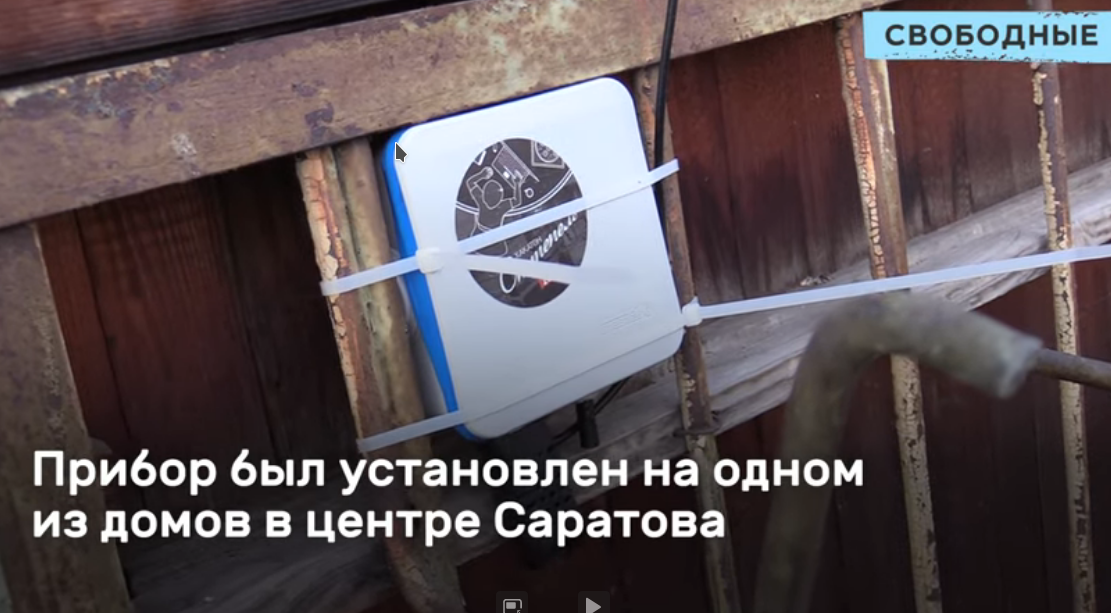
\includegraphics[width=\textwidth]{assets/device.png}
    \end{minipage}
\end{frame}

\section{Радиационная обстановка}
\begin{frame}{\insertsectionhead}

    Радиационная обстановка на территории области стабильная и 
    находится в пределах природного радиационного фона.

    \medskip

    \begin{table}
        \begin{tabular}{|c|c|c|c|c|c|c|}
            \hline
            \textbf{Месяц} &
            05.19 &
            04.19 &
            03.19 &
            02.19 &
            11.19 &
            10.18 \\
            \hline
            \textbf{мкЗв/час} &
            0.09-0.16 &
            0.10-0.15 &
            0.09-0.13 &
            0.09-0.14 &
            0.08-0.17 &
            0.09-0.18 \\
            \hline
        \end{tabular}
        \caption{МЭД за 6 месяцев}
    \end{table}
\end{frame}
